\documentclass{scrartcl}
\usepackage[ngerman]{babel}
\usepackage[utf8]{inputenc}
\usepackage[left=1in,right=0.8in,top=0.5in,bottom=0.5in,includeheadfoot]{geometry}
\usepackage[hidelinks]{hyperref}
\usepackage{graphicx}
\usepackage{subcaption}
\usepackage{float}
\usepackage{color}
\usepackage{listings}
\usepackage{dirtree}
\usepackage{diagbox}
\usepackage[autostyle]{csquotes}
\usepackage{amsmath}
\usepackage{algorithm2e}
\usepackage[backend=biber,style=authoryear,citestyle=authoryear,url]{biblatex}
\bibliography{library.bib}
\lstset{
	language         = Python,
    showstringspaces = false,
    basicstyle       = \small\ttfamily\color{magenta},
    identifierstyle  = \color{black},
    keywordstyle     = \color{red},
    stringstyle      = \color{blue},
    breaklines       = true,
    xleftmargin      = .1\textwidth
}

% space before and after floating element e.g. figures
\setlength{\intextsep}{24pt plus 2.0pt minus 4.0pt}
\setlength{\belowcaptionskip}{-5pt plus 10pt minus 10pt}

% add custom product-number field to litarute
\DeclareSourcemap{
    \maps[datatype=bibtex]{
      \map{
        \step[fieldsource=product-number]
        \step[fieldset=usera,origfieldval]
    }
  }
}

\DeclareFieldFormat{usera}{\texttt{#1}}
\AtEveryBibitem{%
    \csappto{blx@bbx@\thefield{entrytype}}{% put at end of entry
        \iffieldundef{usera}{}{\space[Katalog, Artikelnummer: \printfield{usera}]}
    }
}

\renewcommand{\baselinestretch}{1.3}
\renewcommand{\lstlistingname}{Code}
\setlength{\parindent}{0in}
\setlength{\parskip}{1.8ex plus 0.2ex minus 0.3ex}

\title{Texteingabe Vorhersage (next word prediction) für Schwerstmehrfachbehinderte}
\author{Manuel Reich}
\date{April 2015}

\begin{document}

	\maketitle
	\newpage
	
    %table of contents
    \pagenumbering{roman}
    \setcounter{page}{1}
	\tableofcontents
	\newpage

	%content
    \pagenumbering{arabic}
    \setcounter{page}{1}

	\section{Einleitung}
UK erklären
vielleicht next word prediction erklären
\newpage
	\section{Grundlagen}

	\subsection{Eingabegeräte für Schwerstmehrfachbehinderte}
    \label{sec:input-devices}
    
    	Aufgrund der Vielzahl an möglichen Behinderungen und Einschränkungen gibt es eine mindestens genau so große Zahl an Eingabemethoden und Geräten. Diese Eingabegeräte können sowohl eine Schnitstelle zu klassischen PCs darstellen oder auch zur Bedienung von unterstützenden Technologien wie z. B. eines Rollstuhls benutzt werden. Im Folgenden sollen hier exemplarisch einige solcher Eingabegeräte vorgestellt werden. Die hier vorgestellte Auswahl ist nicht vollständig und ist aus den Onlinekatalogen der \emph{RehaMedia GmbH}, und der \emph{REHAVISTA GmbH} sowie den Webseiten der erwähnten Hersteller zusammengetragen.
        
        \subsubsection*{Augensteuerung}
        	Bei der Augensteuerung werden mit Hilfe einer Kamera die Bewegungen der Augen genutzt um ein Gerät zu steuern. Damit können dann auch Windows oder OS X Betriebssysteme mit Hilfe eines On-Screen-Menüs gesteuert werden. Der Anbieter \emph{RehaMedia} bewirbt das System \emph{Tobii PCEye} mit den Worten:" \enquote{Die Augensteuerung erfasst die Augenbewegungen und setzt sie präzise in Mausbewegungen um. Dank eines Mauszeigermenüs stehen auch bei der Bedienung mit der Augensteuerung alle Mausfunktionen wie Doppelklick, Rechtsklick usw. zur Verfügung."} \parencite{rehamedia:TobiiPCEyeGo}
            
         \subsubsection*{Taster}
         	In der Regel handelt es sich bei Tastern um einen einzelnen großen runden Knopf (\autoref{fig:bigRed}). Es gibt aber auch andere Ausführungen wie einen Griff, welchen man zusammendrücken kann oder einen befestigten Stab, gegen den man Druck ausüben kann. Manche Taster können auch an der Kleidung oder an einer Kopfstütze angebracht werden, so dass eine Bedienung nicht nur mit den Händen, sondern auch mit dem Kopf oder durch  Zusammenschlagen der Knie möglich ist. Pedale zur Bedienung mit den Füßen werden auch angeboten. Die meisten Taster verwenden einen 3,5 mm Klinkenstecker und können damit ein einziges Signal (Knopf gedrückt) senden. Der Hersteller \emph{ablenet} bietet z. B. Spielsachen an, die so gesteuert werden können (\autoref{fig:penguinRace}). Andere Eingabegeräte können auch Anschlüsse für diese Taster bereitstellen so dass diese kombiniert werden können.  
         	
            \begin{figure}[H]
				\centering
				\begin{subfigure}{.49\textwidth}
  					\centering
  					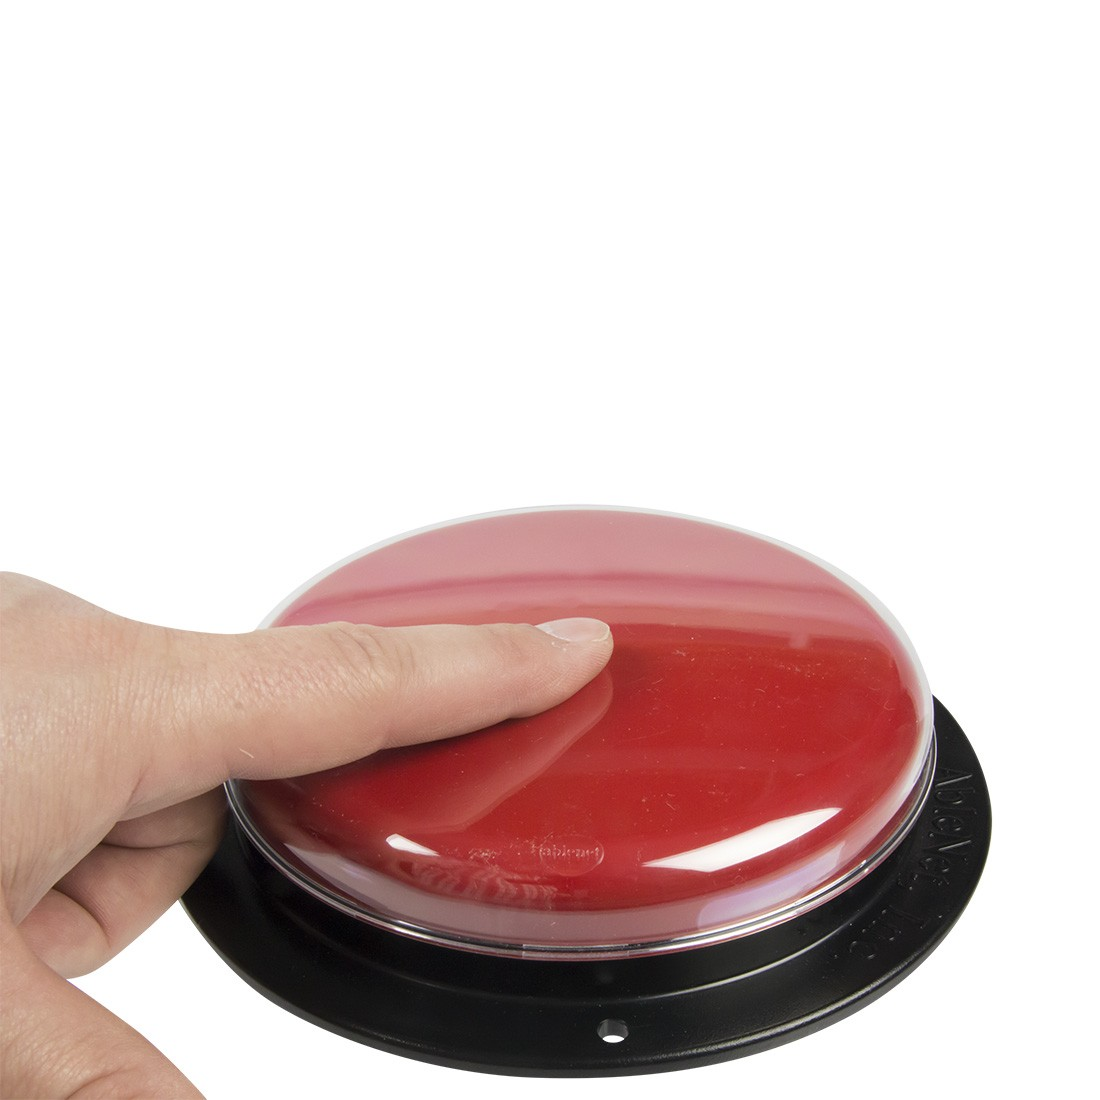
\includegraphics[width=.8\linewidth]{images/big-red-button.jpg}
  					\caption{\emph{Big Red} \cite{ablenet:bigRed}}
                    
  					\label{fig:bigRed}
				\end{subfigure}
				\begin{subfigure}{.49\textwidth}
  					\centering
  					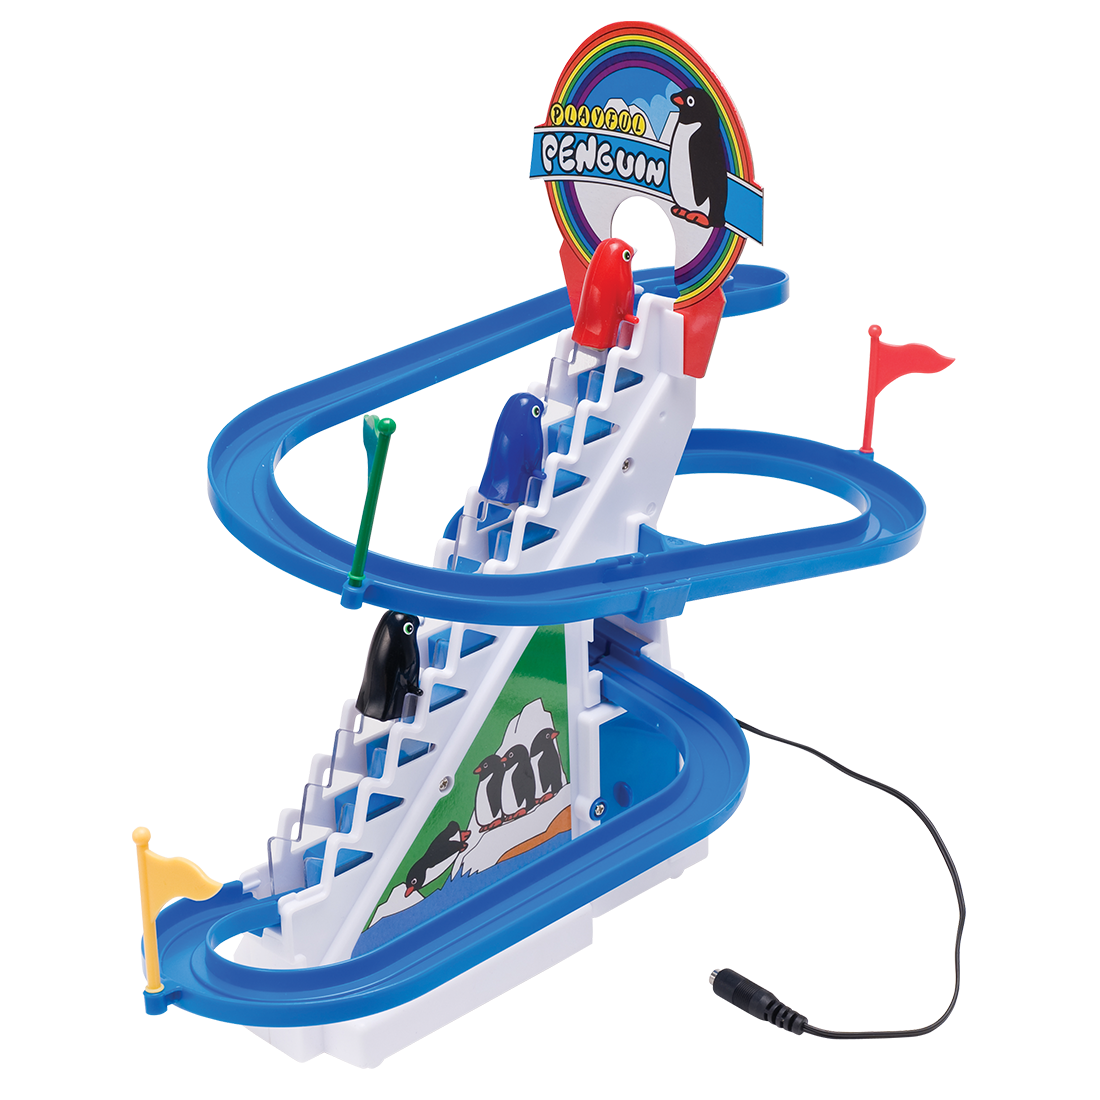
\includegraphics[width=.8\linewidth]{images/penguin-race.png}
  					\caption{\emph{Penguin Race} \cite{ablenet:penguinRace}}
  					\label{fig:penguinRace}
				\end{subfigure}
                \caption{Taster und Spielzeug von ablenet}
				\label{fig:ablenetSingleButtons}
			\end{figure}
            
            Eine weitere Ausführung sind \emph{sprechende Tasten}. Diese Taster haben einen Lautsprecher eingebaut und bieten die Möglichkeit, eine oder mehrere Sprachnachrichten aufzunehmen. Wenn mehrere Nachrichten aufgenommen werden können, kann die auszugebende Nachricht von einer betreuenden Person voreingestellt werden. Andere Geräte funktionieren nach dem Prinzip: einmal drücken gibt Nachricht Nummer eins aus, zweimal drücken Nachricht Nummer zwei und dreimal drücken Nachricht Nummer drei.
            
        	Außerdem gibt es Taster mit mehr als einer Taste. Diese sind dann schon zum Anschluss an Computer oder Tablets gedacht und haben häufig einen \emph{USB}- oder \emph{Bluetooth}- Anschluss. Der Tastenumfang geht dabei von einfachen Geräten mit zwei Tasten bis zu kompletten Computertastaturen.
            
            \begin{figure}[H]
				\centering
				\begin{subfigure}{.33\textwidth}
  					\centering
  					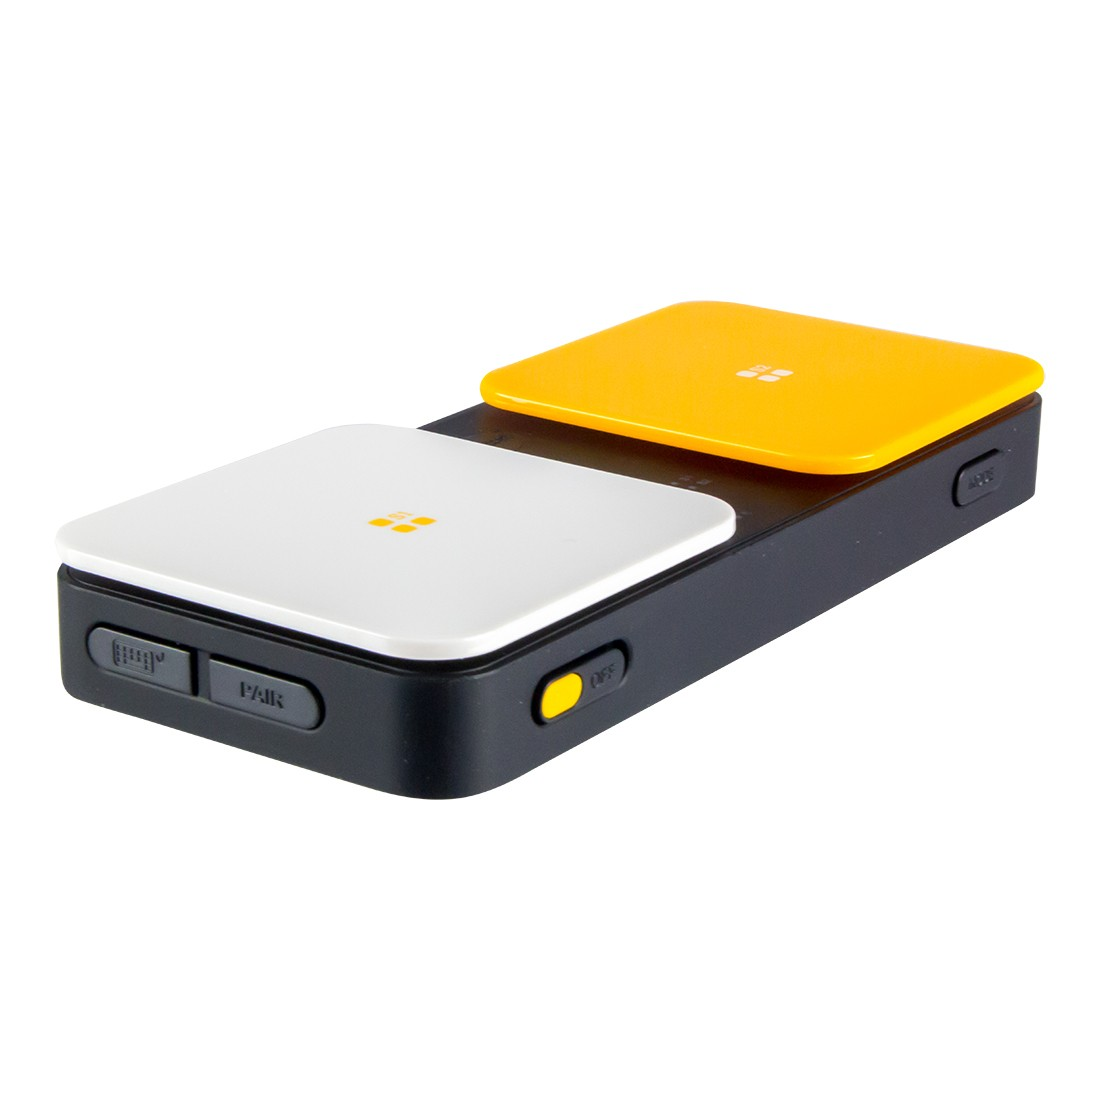
\includegraphics[width=.8\linewidth]{images/buttonsIPad.jpg}
  					\caption{\cite{ablenet:iPad}}
                    
				\end{subfigure}%
				\begin{subfigure}{.33\textwidth}
  					\centering
  					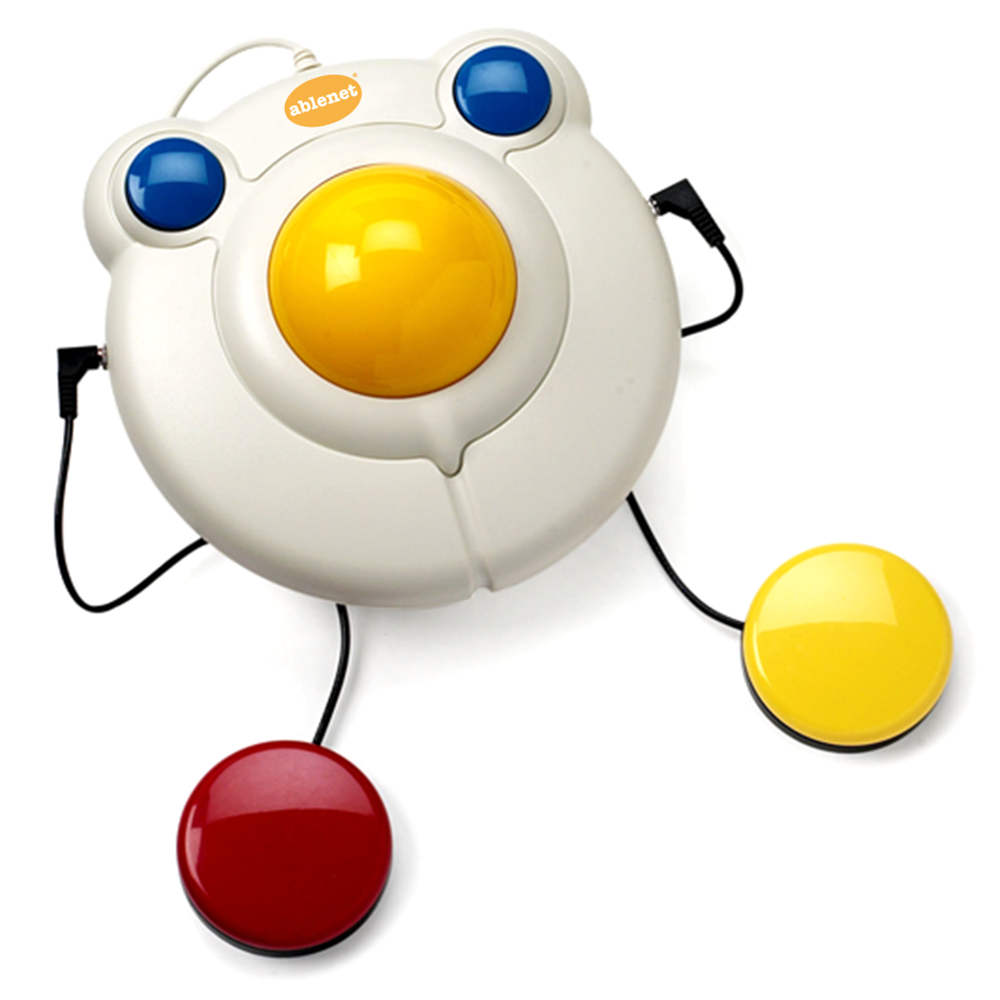
\includegraphics[width=.8\linewidth]{images/buttonsMouse.png}
  					\caption{\cite{ablenet:mouse}}
				\end{subfigure}
                \begin{subfigure}{.33\textwidth}
  					\centering
  					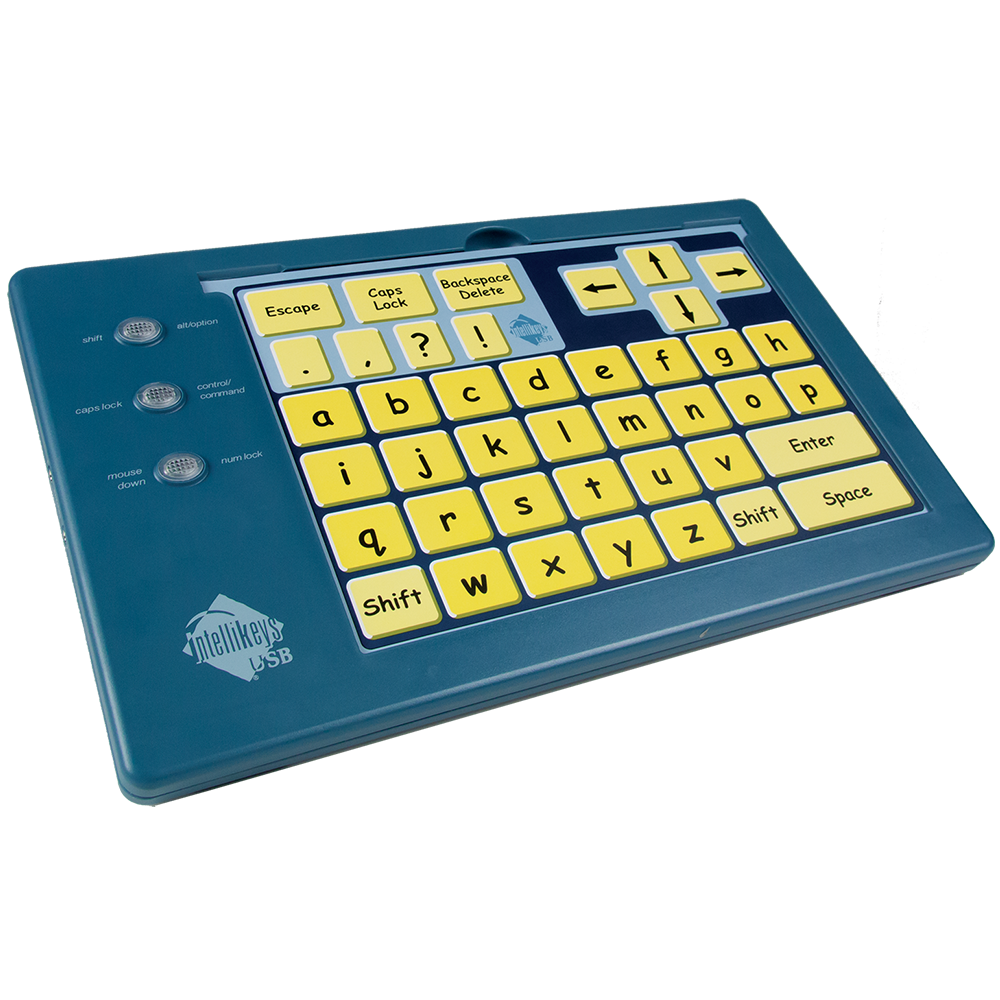
\includegraphics[width=.8\linewidth]{images/buttonsKeyboard.png}
  					\caption{\cite{ablenet:keyboard}}
				\end{subfigure}
                \caption{Taster mit mehreren Tasten von ablenet}
				\label{fig:ablenetMultipleButtons}
			\end{figure}
            
		\subsubsection*{Talker}
        	Bei Talkern handelt es sich um Geräte, mit denen durch Knopfdruck Sprache ausgegeben werden kann. Es existieren sowohl statische als auch dynamische Systeme. Bei statischen Systemen sind die Knöpfe fest in der Hardware eingebaut. Dynamische Systeme verwenden Touchscreens. Oft werden dafür auch handelsübliche Tablets mit Schutzhüllen und Halterungen verwendet. 
            
            Diese Systeme können unterschiedlich komplex sein. Einfachere Talker haben ein festes Set an Symbolen, welche auf Knopfdruck Sprachnachrichten ausgeben. Dynamische Systeme ermöglichen die Navigation durch verschiedene Symbolgruppen oder arbeiten sogar nur mit Text. Manche ermöglichen auch eine Texteingabe per Tastatur. In \autoref{sec:software-examples} werden verschiedene Softwarelösungen für solche Systeme vorgestellt.
            
            \begin{figure}[H]
				\centering
				\begin{subfigure}{.3\textwidth}
  					\centering
  					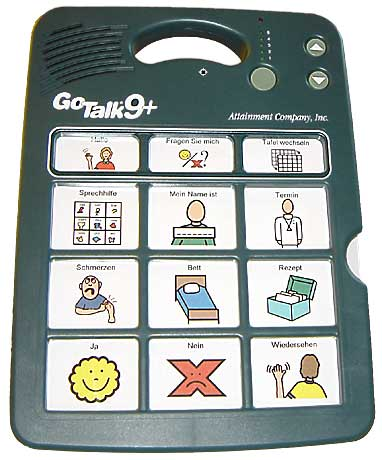
\includegraphics[width=.8\linewidth]{images/goTalkPlus.jpg}
  					\caption{statischer Talker \parencite{rehavista:goTalkPlus}}
                    
				\end{subfigure}
				\begin{subfigure}{.3\textwidth}
  					\centering
  					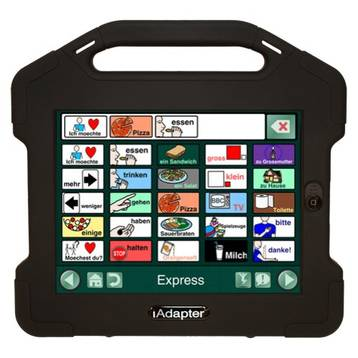
\includegraphics[width=.8\linewidth]{images/goTalkNow.jpg}
  					\caption{iPad mit Talker Erweiterung \parencite{rehamedia:goTalkNow}}
				\end{subfigure}
                \begin{subfigure}{.3\textwidth}
  					\centering
  					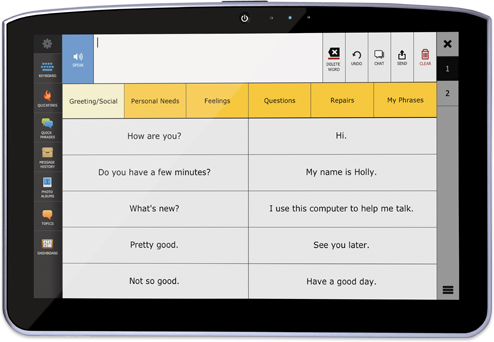
\includegraphics[width=.8\linewidth]{images/tobiiT15.png}
  					\caption{Talker mit literarischem Interface \parencite{tobii:T15}}
                    \label{fig:tobiiT15}
				\end{subfigure}
                \caption{verschiedene Talker}
				\label{fig:talker}
			\end{figure}
            
    \newpage      
    \subsection{Software für Unterstützte Kommunikation}
    \label{sec:software-examples}
    
    	Unter Sprachsoftware wird hier das komplette System von Benutzeroberfläche über mögliche Autovervollständigungen und Eingabevorschlägen bis zur Sprachausgabe verstanden. Im Speziellen soll hier Software vorgestellt werden, die auf den in \autoref{sec:input-devices} beschriebenen \emph{Talkern} Anwendung finden. Die Auswahl der Beispiele richtet sich an ihrer Relevanz für den zu entwickelnden Prototypen. Also Software, deren Funktion den in \autoref{sec:requirements} formulierten Anforderungen nahe kommt.
        
        \subsubsection*{MetaTalkDE / MetaTalkUS}
        	\emph{MetaTalkDE} ist eine iPad App von \emph{Cidar Health Care LLC} für Symbolbasierte \emph{Unterstützte Kommunikation}.
            
            \begin{figure}[H]
				\centering
				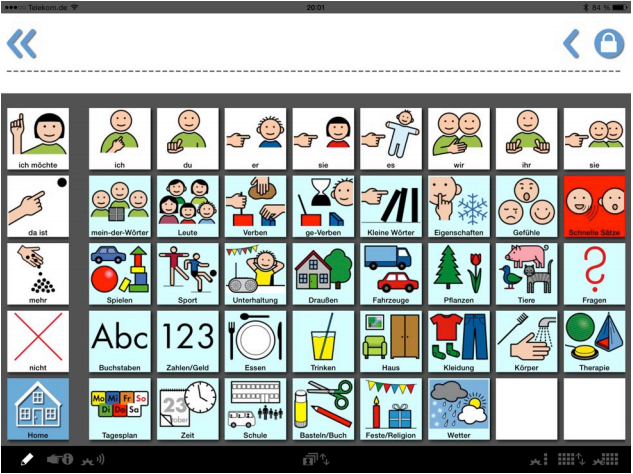
\includegraphics[width=.6\linewidth]{images/Metatalk.png}
                \caption{Schreenshot von MetaTalkDE in der 5x9 Ansicht
                	\parencite[S. 8]{cidar:metaTalkManual}
                }
				\label{fig:metatalk}
			\end{figure}
            
            Auf dem Startbildschirm werden oben in einer Zeile vom Nutzer bereits ausgewählte Symbole angezeigt. Darunter befindet sich ein Raster mit Symbolen und Kategorien. Durch Auswahl einer Kategorie gelangt man auf einen neuen Bildschirm mit entsprechenden Symbolen.
            Durch Druck auf die Symbolzeile oben werden die gelisteten Symbole gesprochen. 
            Laut Handbuch \parencite[S. 7 ff]{cidar:metaTalkManual} ist die Anzahl der Tasten im Raster in drei Stufen (5x9, 4x7, 3x5) anpassbar. Beim Anpassen des Rasters wird auch das Vokabular angepasst. Jede Stufe hat ein eigenes Vokabular, wobei standartmäßig mehr Tasten auch ein größeres Vokabular bedeuten. Die Vokabulare sind innerhalb der App editierbar und können, wie auf Seite 20 f. erklärt, auch über E-Mail ex- und importiert werden. Die gesamte App bietet viele Möglichkeiten der Personalisierung. So können die Symbole der Tasten ausgetauscht werden, neue Tasten hinzugefügt werden, Tasten mit Farben hinterlegt werden und auch Töne für die Sprachausgabe aufgenommen werden (vgl. S.24). Nach Auswahl von Personalpronomen werden die Verben in der passenden Form angezeigt. Dazu lassen sich durch langes Drücken auf ein Symbol andere Formen des entsprechenden Wortes anzeigen. (vgl. S.11 – 14) Auch wird auf Seite 33 erleutert wie sich \emph{Verlinkungen} erstellen lassen, mit denen darauffolgende Symbollisten angezeigt werden.
            
            Da die App auf einem iPad läuft, muss der Nutzer motorisch in der Lage sein, diese mit den Händen zu bedienen. Zwar gibt es die oben beschriebenen \emph{Verlinkungen}, jedoch nutzt die App keine Methoden des \emph{Mashine learning}, um die Eingabe durch optimierte Symbollisten zu erleichtern.
            
        \subsubsection*{Tobii Sono Scribe}
        
        	\emph{Tobii Sono Scribe} ist eine Erweiterung zu der Software \emph{Tobii Communicator}. Die Eingbe ist textbasiert. Das Handbuch \parencite[S. 8]{tobii:sonoScribeManual} beschreibt zwei verschiedene Modi. In einem Modus wird mit einer Liste von vorgeschlagenen Wörtern gearbeitet (\autoref{fig:sonoScribeWords}), in dem anderen wird eine Displaytastatur zur Texteingabe verwendet (\autoref{fig:sonoScribeKeyboard}).
            
            \begin{figure}[H]
				\centering
				\begin{subfigure}{.49\linewidth}
  					\centering
  					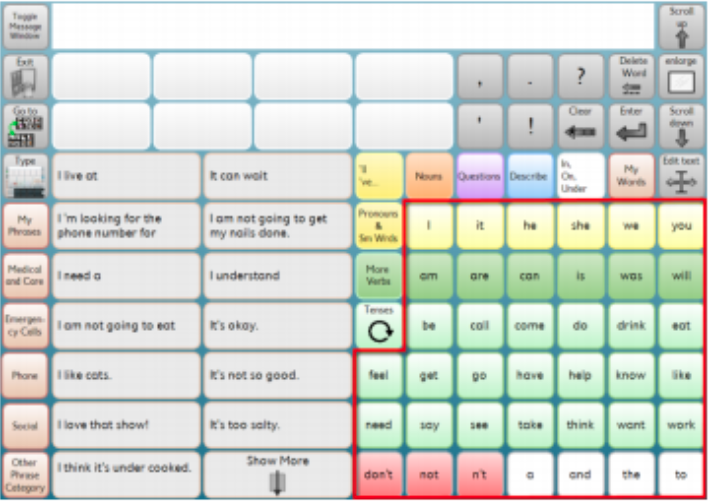
\includegraphics[width=.8\linewidth]{images/sonoScribeWords.png}
  					\caption{Wort Modus 
                    	\parencite[S. 13]{tobii:sonoScribeManual}
                    }
                    \label{fig:sonoScribeWords}
				\end{subfigure}
				\begin{subfigure}{.49\linewidth}
  					\centering
  					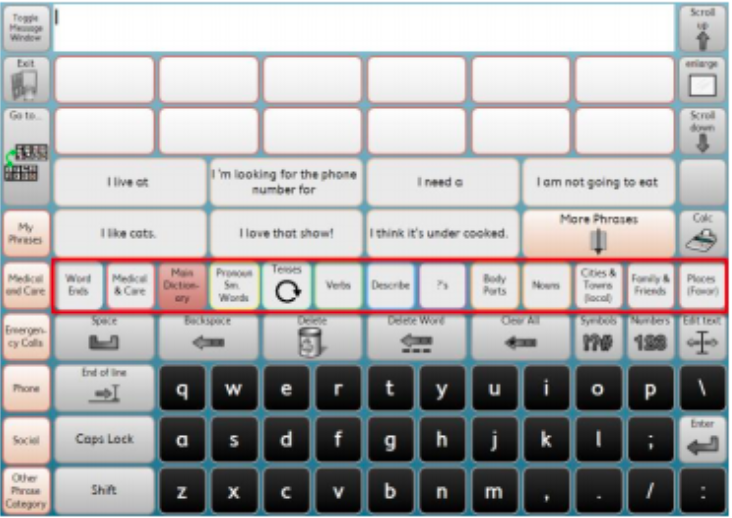
\includegraphics[width=.8\linewidth]{images/SonoScribeKeboard.png}
  					\caption{Tastatur Modus 
                    	\parencite[S. 22]{tobii:sonoScribeManual}
                    }
                    \label{fig:sonoScribeKeyboard}
				\end{subfigure}
                \caption{ }
                \label{fig:sonoScribe}
			\end{figure}
        	
            Die Software kann unter Windows und auf den Geräten von \emph{Tobii} installiert werden. Zum Beispiel auf dem in \autoref{fig:tobiiT15} gezeigtem \emph{T15}. Neben dem enthaltenen Vokabular werden auch verschiedene Listen mit häufig verwendeten Sätzen angeboten, wie auf S. 15 f des Handbuchs beschrieben wird. Sowohl die Sätze, als auch, wie auf S. 20 ergänzt, das Vokabular, sind innerhalb der Software editierbar.
            
            Bei der Eingabe werden wie auf S. 15 beschrieben, mögliche nächste Wörter vorgeschlagen und auch Sätze mit entsprechenden Anfängen aus den gespeicherten Sätzen vorgeschlagen. Im tastaturbasierten Modus werden auch Wortvervollständigungen angeboten (Siehe S. 22). Auf S. 18 wird erklärt, dass Nutzer sich, wie in \autoref{fig:sonoScribeList} zu sehen, auch Listen von Wörtern sortiert nach der Wortart anzeigen lassen können.
            
            \begin{figure}[H]
  				\centering
  				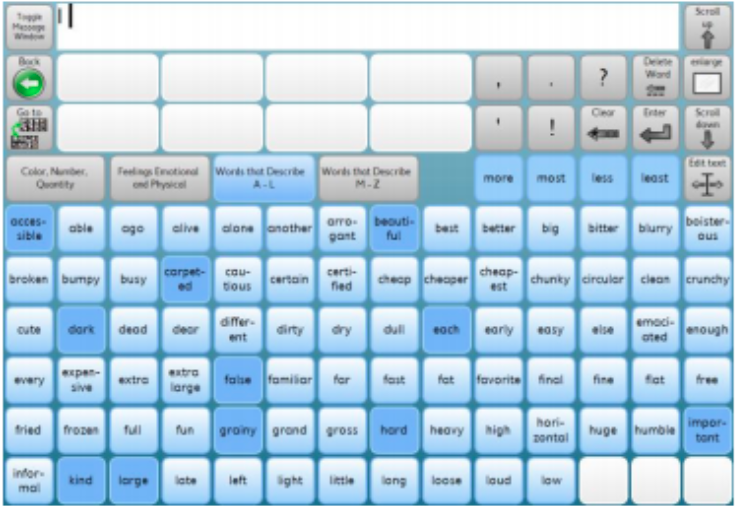
\includegraphics[width=.6\linewidth]{images/SonoScribeList.png}
  				\caption{Liste von Nomen \parencite[S. 18]{tobii:sonoScribeManual}}
                \label{fig:sonoScribeList}
			\end{figure}
            
			Neben der Sprachausgabe gibt es auch einen Texteditor, einen Mailclienten, sowie verschiedene Tools zur Steureung des Windows Betriebssystems. Dazu gehört auch ein PlugIn für den Browser \emph{Mozilla Firefox}. Diese große Anzahl an Funktionen setzt aber voraus, dass Nutzer lesen und schreiben können müssen und fähig sind, die im Vergleich mit \emph{MetaTalkDE} komplexe Benutzeroberfläche bedienen zu können. Die Software unterstützt unter anderem die Eingabe per Touch, Augensteuerung und sogar durch Taster. Bei der Bedienung mit Taster gibt es ein \emph{Scan Raster}, nach dem per Tastendruck von Knopf zu Knopf gesprungen wird.
    
    \newpage
	\subsection{Mashine learning Software für den Massenmarkt}
    \emph{Mashine learning} zur Wortvorhersage wird nicht nur in der \emph{Unterstützten Kommunikation} angewendet, sondern auch in der Software für den Massenmarkt. Im Folgenden sollen hier kurz drei Beispiele vorgestellt werden, die Nutzern Worte zur Eingabe vorschlagen.
        
        \subsubsection*{swiftKey}
        	In einem Artikel für die Webseite \emph{techrepublic.com} beschreibt \cite{techrepublic:swiftKey} die Funktionen der Bildschirmtastatur für mobile Geräte \emph{swiftKey}. Zuerst erwähnt er, wie Nutzern dank eines lernfähigen Algorythmus Worte vorgeschlagen werden. Im optimalen Fall müsste man also nach Eingabe des ersten Wortes gar nicht mehr tippen. Dann beschreibt er die zweite Funktion, welche \emph{Flow} genannt wird. Hierbei wird zum Tippen nicht abgesetzt, sondern mit dem Finger von einem Buchstaben zum anderen gewischt. Die Tastatur kann auch so das gewünschte Wort erkennen.
        
        
        \subsubsection*{iOS QuickType}
        
        	Die Bildschirmtastatur für \emph{Apple iOS 8} enthält ein Feature mit dem Namen \emph{QuickType}. Die Funktion ist ähnlich zu \emph{swiftKey}. Auch hier werden beim Tippen Worte vorgeschlagen. \emph{Apple} bewirbt auf seiner Webseite, dass die Wortvorschläge Kontextabhängig sind. So wird beschrieben, dass in einem Mailprogramm andere Worte vorgeschlagen werden, als in einem Chat mit einem Freund. Außerdem kann die Tastatur laut \cite{apple:quickType} auch einen eingehenden Text in einer Chatapplikation analysieren und entsprechende Vorschläge für die Antwort machen. Eine Funktion zum Tippen ohne abzusetzen gibt es nicht.
        
        \subsubsection*{Google Suggest}
        
        	Auch \emph{Google} schlägt Nutzern Worte vor, während diese Begriffe in die Suchmaschine eingeben. Dieser Service nennt sich \emph{Google Suggest}. Dies beschreibt \cite{google:suggestIntro} im offiziellen Blog von Google. Außerdem erwähnt sie, dass der Service auch Rechtschreibfehler verbessern kann. In einem anderen Blogeintrag erklärt \cite{google:suggestUpdate}, dass \emph{Goggle} 2\% die eingegeben Suchanfragen zusammen mit der IP-Adresse des Nutzers auswertet und aus diesen Daten die Vorschläge generiert.
    
    
    
    \newpage
	\section{Anforderungen}
    
	\subsection{Eingabe}
    	Ziel dieser Arbeit ist die Entwicklung eines Prototypen einer Sprachapplikation. Mit dieser Applikation soll ein stummer und motorisch eingeschränkter Nutzer Sätze erzeugen können, die per Sprachausgabe ausgegeben werden können. Dabei soll es nicht nötig sein zu tippen. Sätze werden erzeugt indem ein Wort nach dem anderen aus einer Liste von Wörtern ausgewählt wird. Am Ende wird der Satz bestätigt und ausgegeben. Sollte ein Wort ausversehen zum Satz hinzugefügt worden sein soll es möglich sein diesen Fehler zu korrigieren und das Wort wider aus dem Satz zu entfernen. Das erste Wort in der Liste ist dabei das Wort welches am wahrscheinlichsten als nächstes im aktuellen Satz vorkommen wird. Alle weiteren Wörter sind dann nach absteigender Wahrscheinlichkeit sortiert.
         
    	Dieses Kapitel befasst sich mit den Anforderungen bezüglich der Eingabe die sich an die Applikation stellen. Aufgrund der Vielzahl an möglichen Behinderungen und Einschränkungen gibt es eine mindestens genau so große Zahl an Eingabemethoden und Geräten. In vielen Fällen sind Eingabegerät und Software eng miteinander verbunden oder sogar ein in sich abgeschlossenes System.
        
        Um möglichst viele verschiedene Eingabegeräte zu unterstützen soll die zu entwickelnde Applikation nicht direkt auf spezielle Geräte angepasst werden. Darum werden hier nicht bestimmte Aktionen zur Eingabe beschrieben sondern Signale welche dann von verschieden Geräten erzeugt werden können. Ein Signal kann jeder diskreter Code sein der von einem Eingabegerät an die Software gesendet werden kann. Beispielsweise das Drücken einer bestimmten Taste auf einer Tastatur. Für die Entwicklung des Prototypen sollen Signale dann auch über die Tastatur erzeugt werden. Es ist auch denkbar komplizierte Eingabemethoden zu implementieren um die tatsächliche Nutzerfreundlichkeit besser darzusetllen. Schließlich ist das Tippen einer Taste doch sehr viel einfacher als z. B. das Betätigen eines Kopfschalters an einem Rollstuhl. 
        
        Da nicht jedes Eingabegerät die gleiche Anzahl an Signalen liefert soll hier ein Minimum von drei diskreten Signalen festgelegt werden. Mit diesen drei Signalen sollen alle Funktionen der Applikation umzusetzen sein. Dabei ist es möglich, dass das gleiche Signal in einem anderen Kontext eine andere Bedeutung hat. Es ist auch vorstellbar, wenn unbedingt nötig, eine weitere Funktion durch Wiederholen des gleichen Signals innerhalb eines gewissen Zeitraums aufzurufen. Diese Einschränkung wäre natürlich für Nutzer von Eingabegeräten welche mehr als drei Signale erzeugen können schnell frustrierend. So soll es möglich sein auf weitere Signale zu reagieren und mit diesen Erleichterungen in der Bedienung der Applikation umzusetzen. Ein Beispiel hierfür wäre eine Liste, die sich über mehrere Zeilen erstreckt. Es ist möglich durch diese mit einem einzigen "weiter" Befehl zu navigieren. Wenn möglich wäre es aber auch wünschenswert eine Zeile nach unten oder eben auch zurück zu navigieren.
        
        Bei der Betrachtung bestehender Eingabegeräte fallen weitere Anforderungen an die Bedienung der Applikation auf. Es gibt verschiedene Eingabegeräte die zur Steuerung eines Mauszeigers gedacht sind. Meist scheint hier die Bedienung der Maus etwas komplizierter als mit einer klassischen Computermaus. Andere Geräte arbeiten mit verschieden angeordneten großen Tasten, manche bilden diese Tasten auch auf einem Touchscreen ab. Darum sollte es auch möglich sein die Schaltflächen der Applikation klassisch per Maus oder Fingerdruck auswählen zu können. Dabei sollte auf die ungewöhnliche Steuerung des Mauszeigers oder motorische Einschränkungen bei der Bedienung von Touchscreens Rücksicht genommen werden.
        
        Ziel dieser Abstrahierung der Eingabehandhabung ist zum einen die Konzentration der Arbeit und des Prototypen auf die Sprachanalyse und die Visualisierung der Ergebnisse. Zum Anderen aber auch der Versuch die Grundlagen für ein Modulares System zu skizzieren welches auch mit zukünftigen noch nicht existierenden Eingabegeräten funktionieren kann. Ein Beispiel hierfür wäre der bereits erwähnte Mauszeiger der eben nicht nur über eine klassische Maus gesteuert werden kann sondern unter anderem auch mit Trackpad, Trackball oder Trackpoint.
        \newpage
        
        
        
	\subsection{Kathegorie-auswahl / -erkennung}
    	Da zur Prädiktion von wahrscheinlichen nächsten Wörtern zuerst einmal ein Satzanfang benötigt wird startet man zu Beginn mit einer Kategorieübersicht. Hier sollen die Kategorien auch als Liste dargestellt werden. Basierend auf der Kategorieauswahl soll nun eine Liste von möglichen Satzanfängen oder möglichen ersten Wörtern eines Satzes angezeigt werden. 
        
        Durch die enorme Einschränkung der möglichen Eingabesignale kann das navigieren durch lange Listen sehr zeitaufwändig werden. Natürlich stehen im optimalen Fall die benötigten Wörter am Anfang der Liste. Es ist aber zu erwarten, dass es immer wieder Fälle gibt bei denen keine sinnvolle oder hilfreiche Prädiktion gemacht werden kann. Um in diesem Fall immer noch eine einigermaßen überschaubare und sinnvolle Liste erstellen zu können, soll der Wortschatz der Kategorie entsprechend eingeschränkt werden. Dabei ist es denkbar mit Unterkategorien zu arbeiten welche automatisch aufgrund der Vorherigen Sätze bestimmt werden. Diese Unterkategorisierung soll im Hintergrund vom Nutzer unbemerkt stattfinden.
        
        Oberkategorien dagegen werden vom Nutzer bewusst und manuell ausgewählt. Auch soll es zu jeder Zeit möglich sein die bestehende Oberkategorien zu wechseln um somit Zugang zu einem anderen Wortschatz zu erhalten.
        
        -> irgendwas zur Bestimmung von Kategorien
        \newpage
        
        
       	\subsection{Ausgabe}
        
        -> Oben Satz unten Wörter
        -> sehr reduziertes interface
        -> Nach auswahl eines Worts wird neue Liste generiert
        -> Liste als raster von buttons
        -> color coding von Wortarten?
        -> konjugierung nach Eigabe ?
        -> sprachausgabe nicht teil der Arbeit da trivial
        -> Applikation in englischer Sprache
        -> skalierbar aber konzipiert für typische tablets
           also c.a. DinA4
        -> "zurück Button" zur Kategorieauswahl auf Listeposition -1
        -> max 70 Wörter -> alles darüber zu Zeitaufwändig schnelle  
           Bedienug über kompletter Wortschatz
    
    
    
    
    
    
    
    
    
    
    
    
    
    
    
    
    
    
    
    
	\section{Design}
	
    \subsection{Aufbau}
    	In diesem Abschnitt wird der Aufbau des Prototypen erklärt. Man kann sich den Prototypen aufgegliedert in die folgenden drei wesentliche Teile vorstellen:
            
		\begin{description}
			\item[Kivy] ist der Name des verwendeten \emph{frameworks} und vor allem für die Benutzeroberfläche und für das Verarbeiten von Benutzereingaben verantwortlich. Es dient als Rahmen der Applikation und ist für die Kommunikation mit dem jeweiligen Betriebssystem zuständig.
        
        	\item[Learner und Predictor] sind für den \emph{Natural Language Processing} Teil der Anwendung zuständig. Der \emph{Learner} kann neue Sprachmodelle aus Texten erzeugen. Der \emph{Predictor} kann mit Hilfe dieser Sprachmodelle Wortlisten generieren. 
        
        	\item[Adapter] bilden Signale von verschiedenen Eingabegeräten auf die vom Prototypen definierten Signale ab. Sie ermöglichen es \emph{Plugins} für weitere Eingabegeräte zu schreiben.
		\end{description}
        
        \begin{figure}[H]
			\centering
            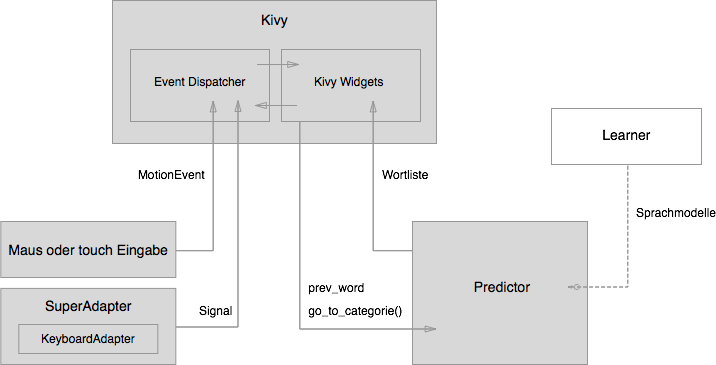
\includegraphics[width=.8\linewidth]{images/aufbau.png}
            \caption{Aufbau des Prototypen}
            \label{fig:architecture}
        \end{figure}
    
    \newpage
	\subsection{Kivy}
    	Die Software ist in \emph{Python} geschrieben. \emph{Python} scheint eine viel für \emph{Natural Language Processing} verwendete Sprache zu sein. Sucht man z. B. auf \emph{github.com} nach den in \autoref{tab:githubNLP} gezeigten Begriffen, liegt Python als Sprache immer weit vorne.
        
        \begin{figure}[H]
			\centering
                
			\begin{tabular}{ r || c | c | c}
                \diagbox{Sprache}{Suchbegriff} & NLP & Natural Language & Natural Language Processing \\ \hline \hline
                Python & 1168 & 500 & 348\\ \hline
                Java & 740 & 269 & 172\\ \hline
                JavaScript & 135 & 146 & 37 \\ \hline
                Ruby & 103 & 100 & 28 \\ \hline
                C++ & 76  & 45 & 23 \\ \hline
            \end{tabular}
            \caption{Anzahl gefundener Repositories in den top fünf Sprachen für die entsprechenden Suchbegriffe auf \texttt{https://github.com/search} (besucht am 02.07.2015)}
			\label{tab:githubNLP}
		\end{figure}
        
        Für \emph{Python} gibt es viele verschiedene \emph{frameworks} zur Erstellung von grafischen Benutzeroberflächen. Eine Liste davon findet sich unter \texttt{https://wiki.python.org/moin/GuiProgramming}.
        
        Für den Prototypen wird ein \emph{open source framework} mit dem Namen \emph{Kivy} verwendet. Laut der offiziellen Webseite \parencite{kivy:homepage} laufen mit \emph{Kivy} geschriebene Applikationen unter Linux, Windows, OS X, Android und iOS. Dazu muss die Applikation für jedes entsprechnende System gepackt werden.
        
		Wie in der Dokumentation unter \cite{kivy:events} beschrieben wird, fasst \emph{Kivy} verschiedene \emph{Input events} als \texttt{MogtionEvent} zusammen. Für einen Button macht es keinen Unterschied, ob er mit einer Maus geklickt oder mit dem Finger gedrückt wurde.
        
        \emph{Kivy} stellt auch eine eigene \texttt{EventDispatcher} Klasse zur Verfügung. Diese steuert die Signale von \emph{touch}- oder Mauseingaben, sowie Signale, die von den \emph{Adaptern} gesendet werden. Eine \emph{Kivy} Applikation besteht aus sogenannten \emph{widgets}. Wie in der Dokumentation unter \cite{kivy:widgets} erklärt, hat ein \emph{widget} einen \emph{Canvas} in welchem gezeichnet werden kann. Es kann auf \emph{events} reagieren und diese selbst senden. \emph{Widgets} sind als \emph{tree} organisiert und jede Applikation benötigt zumindest ein \emph{root widget}
        
        Im \emph{root widget} des Prototypen befinden sich \emph{handler} für die Signale, die von den \emph{Adaptern} gesendet werden können. Außerdem wird hier eine Instanz des \texttt{WordPredictor}s erzeugt, von welcher Kategorien und Wortlisten generiert werden. Dazu wird dem \texttt{WordPredictor} durch einen Aufruf von \texttt{go\_to\_categorie()} die von Nutzer gewählte Kategorie mitgeteilt. Und nach jeder Wortauswahl wird das ausgewählte Wort \texttt{prev\_word} an den \texttt{WordPredictor} gesendet. Siehe \autoref{fig:architecture}.
        
	\subsection{Learner und Predictor}
    \label{sec:design-learnerPredictor}
    
    	Der \emph{Learner} besteht aus zwei speraten Teilen. Aus einem \emph{Tokenizer} und einem \emph{Clusterer}. Der \emph{Tokenizer} hat die Aufgabe, Texte wie sie z.B. in einem Buch zu finden sind, zu bereinigen. Dem \emph{Tokenizer} werden mehrere Textdateien übergeben, aus welcher dieser eine einzelne neue Textdatei generiert. Darin befindet sich der bereinigte Text in einer Form, wie er von dem \emph{Clusterer} gelesen werden kann.

		Der \emph{Clusterer} liest und analysiert die vom \emph{Tokenizer} generierte Textdatei. Dieser Umweg über eine extra generierte Datei ist nötig, da für den \emph{Clusterer} eine \emph{third party} Lösung verwendet wird. Dies wird in \autoref{sec:thirdTry} genauer beschrieben. In erster Linie gruppiert der \emph{Clusterer} die übergebenen Worte in Klassen und speichert das Ergebniss wieder in mehreren Dateien ab. Diese Dateien enthalten neben den Wortklassen auch die Information, wie oft ein bestimmtes Wort nach einem anderen kommt. Die vom \emph{Clusterer} generierten Dateien werden im folgenden \emph{Sprachmodell} genannt.

		Das generieren von \emph{Sprachmodellen} ist nicht Teil der gepackten Applikation. Dazu muss für jedes neue Sprachmodell der \emph{Tokenizer} und der \emph{Clusterer} von Hand aufgerufen werden. Das generierte \emph{Sprachmodell} wird dann in den dafür vorgesehen Ordner in der Applikation gelegt.

		In der laufenden Applikation kann der Nutzer eine Kategorie auswählen. Diese entspricht immer einem \emph{Sprachmodell}. Nach der Auswahl wird dieses automatisch von dem \emph{Predictor} geladen. Dieser Prozess wird in \autoref{sec:implemetation-wordPredition} genauer beschrieben. Aufgrund des Sprachmodells wird vom \emph{Predictor} dann eine Wortliste generiert.
       
    \subsection{Adapter}
    	Wie in \autoref{sec:requirements-input} gefordert, ist es möglich, die Applikation ausschließlich mit den drei Signalen \texttt{left}, \texttt{right} und \texttt{enter} zu bedienen. Abgesehen von der Eingabe per \emph{touch} oder mit der Maus reagiert die Applikation nicht direkt auf Eingaben von z. B. der Tastatur sondern nur auf die in \texttt{SuperAdapter} beschriebenen Signale.  
    
    	Ein \emph{Adapter} besteht aus einer einzigen \emph{Python} Datei mit dem Namen des Gerätes, für das er geschrieben wurde, kombiniert mit dem Wort \emph{Adapter}. Jeder \emph{Adapter} muss von der Klasse \texttt{SuperAdaper} erben. \texttt{SuperAdaper} wiederum erbt von \emph{Kivy}'s \texttt{EventDispatcher}.
So ist es einfach innerhalb der Applikation auf Signale zu reagieren. Ein \emph{Adapter} muss der Applikation mitteilen können, ob das dazugehörige Gerät verfügbar ist. Sollte das nicht der Fall sein, wird ein \emph{Adapter} nicht geladen.

		Des weiteren muss ein \emph{Adapter} minimal die drei Signale \texttt{left}, \texttt{right} und \texttt{enter} senden können. Wenn möglich kann ein Adapter auch noch weitere Signale senden. Mögliche weitere Signale sind: \texttt{up}, \texttt{down}, \texttt{talk} und \texttt{close}.
        
        Jeder neue \emph{Adapter} muss in dem Ordner \texttt{inputAdapters} gespeichert werden. Außerdem muss dieser in der \texttt{\_\_init\_\_.py} im gleichen Ordner importiert und in die Liste \texttt{adapters} eingetragen werden. Durch diesen Prozess wird erreicht, dass für das Hinzufügen von einem \emph{Adapter} nur Änderungen innerhalb eines einzigen Ordners vorgenommen werden müssen. Adapter leben also getrennt von der Applikation in einem eigenen Modul. Um einen Adapter zu schreiben, müssen lediglich die oben genannten Anforderungen eingehalten werden. Es sind keine weiterem Kenntnisse über die interne Funktionsweise des Prototypen nötig. Ein System zum Einbinden von externen Adaptern in eine gepackte Applikation existiert allerdings nicht.
	
    \newpage
    \section{Sprachmodelle}

	\subsection{Überblick}
\label{sec:langmodels}

    In diesem Abschnitt sollen die theoretischen Aspekte der Wortvorhersage erleutert werden. Es handelt sich hier um das Themengebiet des \emph{Natural Language Processing}. In diesem Abschnitt werden dazu ausschließlich Sprachmodelle behandelt. Um Annahmen darüber zu machen, welche Wörter nach einem anderen folgen können, benötigt man zunächst einmal ein Modell der verwendeten Sprache. Im optimalen Fall kann ein \emph{Sprachmodell} eine Sprache und die Beziehung zwischen Wörtern umfassend abbilden. In \autoref{sec:design-learnerPredictor} wird ein \emph{Sprachmodell} als Sammlung von Dateien mit Informationen über einen Text definiert. In diesem Abschnitt geht es um die Bedeutung dieser Informationen.
        
    Eine naheliegende Möglichkeit ein Modell einer Sprache zu generieren ist das Formulieren einer \emph{Grammatik}. Hierbei wird versucht die sytaktischen Regeln einer Sprache zu definieren. Im entworfenen Prototypen spielen solche \emph{Grammatiken} keine Rolle. Darum werden diese nur sehr kurz erklärt.
        
    Ein Beispiel einer einfachen Grammatik ist in \autoref{fig:grammer} zu sehen. \texttt{S -> NP VP} beschreibt, dass ein Satz \texttt{S} aus einem \emph{Noun Phrase} \texttt{NP} und einem \emph{Verb Phrase} \texttt{VP} bestehen kann. Alle weiteren Regeln funktionieren entsprechend. Mit Hilfe einer solchen Grammatik ist es möglich die Funktion eines Wortes innerhalb von einem Satz zu bestimmen. Dieser kann dann, wie in \autoref{fig:parsingTree} zu sehen,  als \emph{tree} dargestellt werden. Im Beispiel gilt es zu beachten, dass \autoref{fig:grammer} nicht alle in \autoref{fig:parsingTree} enthaltenden Worte enthält und somit erst einmal nicht funktionieren würde.
        
    Folgen wir also folgender vereinfachten Regel: Innerhalb eines \emph{Preposition Prase} \texttt{PP} nach einer Preposition \texttt{P} und einem Determinator \texttt{DET} muss immer ein Nomen \texttt{N} kommen. Dann können wir in dem Satzteil \texttt{in the …} aus \autoref{fig:parsingTree} nur noch Nomen als Folgewort vorschlagen.
        
    \begin{figure}[H]
		\centering
        \begin{subfigure}{0.49\textwidth}
			\begin{lstlisting}
S -> NP VP
VP -> V NP | V NP PP
PP -> P NP
V -> "saw" | "ate" | "walked"
NP -> "John" | "Mary" | "Bob" | Det N | Det N PP
Det -> "a" | "an" | "the" | "my"
N -> "man" | "dog" | "cat" | "telescope" | "park"
P -> "in" | "on" | "by" | "with"
    		\end{lstlisting}
            \caption{Einfache Grammatik}
            \label{fig:grammer}
		\end{subfigure}
        \begin{subfigure}{0.49\textwidth}
           	\centering
          	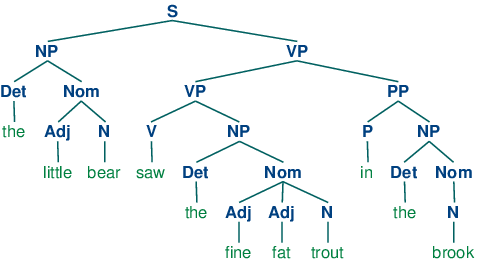
\includegraphics[width=.8\linewidth]{images/grammer.png}
           	\caption{\emph{parsing tree}}
           	\label{fig:parsingTree}
        \end{subfigure}
        \label{fig:grammerWithTree}
        \caption{Beispiel einer einfachen \emph{Grammatik} \parencite[Kapitel 8]{nltk:book}}
        \end{figure}
        \newpage
        
        Allerdings stößt man, wie von \cite[S. 544]{jamia:introduction} im Abschnitt \emph{The limitations of hand-written rules: the rise of statistical NLP} aufgefürht wird, mit solchen \emph{Grammatiken} an Grenzen. In dem Artikel werden zwei Probleme solcher \emph{Grammatiken} beschrieben.
    
    	Zum einen beschreiben diese in erster Linie Syntax und nicht die Semantik eines Satzes. Dies kann laut \cite{jamia:introduction} zwar durch Erweitern der Regeln gelöst werden. Sie Nutzen hier das Beispiel, dass das Verb \texttt{essen} nur für bestimmte \emph{essbare} Nomen gültig gemacht werden kann. Weißen aber darauf hin, dass so die Regeln viel zu komplex und unüberschaubar würden.
        
        Als zweites Problem führen sie an das solche \emph{Grammatiken} mit Sätzen, die zwar von Menschen verstanden werden aber nicht unbedingt grammatischen Regeln folgen, nicht umgehen können.
        
        \cite{jamia:introduction} beziehen sich bei Ihren Überlegungen, auch wenn sie Anwendungsbeispiele aus der Medizin nutzen, auf \emph{Natural Language Processing} im Allgemeinen. Hier soll versucht werden diese Formulierungen bezüglich der Wortvorhersage zu verwenden.
        
        Aufgrund der genannten Probleme gab es, wie \cite{jamia:introduction} auf Seite 545 schließen, in den 1980ern eine Wende hin zu \emph{statistischem Natural Languge Processing}. Sie erklären \enquote{[\dots]fewer, broader rules replace numerous detailed rules, with statistical-frequency information looked up to disambiguate.} Übersetzt meinen sie also, dass weniger aber weiter gefasste Regeln in Kombination mit statistischen Frequenzen detaillierte Regeln ersetzen. Ein Beispiel für solche statistische Modelle sind die in \autoref{sec:n-gramms} erklärten \emph{N-gramms}.
        
        Ein statistisches Modell basiert immer auf Wahrscheinlichkeiten. Im gleichen Abschnitt beschreiben \cite{jamia:introduction} auch, dass diese Wahrscheinlichkeiten abhängig sind von dem Text aus welchem die Statistiken generiert werden. So liefert vereinfacht Formuliert eine auf Prosa Texten gelernte Statistik keine guten Ergebnisse auf Wissenschaftliche Texte.
    \subsection{N-gramms}
    \label{sec:n-gramms}
    
    Um Informationen über ein Wort in einem Text zu erhalten ist eine Möglichkeit sich die Umgebung dieses Wortes anzusehen. Ein \emph{N-gramm} besteht also aus einem Wort und den \emph{N-1} vorherigen Wörtern an einer Textstelle. Mit diesen Informationen können wir auch eine Sprache so beschreiben, dass wir Wortvrhersagen machen können. \parencite[S. 468, Gleichung 1]{cumpatationalLinguistics:classBasedNGramms} machen dazu die in \autoref{eq:wordChain} gezeigte Annahme.
        
    \begin{equation}
       	Pr(w_1^k) = Pr(w_1) Pr(w_2|w_1) \cdots Pr(w_k|w_1^{k-1})
       	\label{eq:wordChain}
    \end{equation}
       
    Sie betrachten also die Wahrscheinlichkeit eines Wortes abhängig von seinen Vorgängern \(Pr(w_k|w_1^{k-1})\). Und definieren die Wahrscheinlichkeit einer Wortkette \(Pr(w_1^k)\) als Summe dieser Wahrscheinlichkeiten. In dem online Buch \parencite{nlwp:book} wird dazu unter Abschnitt 3.8 eine gute Erklärung geliefert. Zunächst formulieren de Kok und Brouwer die Formel neu mit einem Beispielsatz. Hier wird dazu in \autoref{eq:wordChainWithWords} der Satz \texttt{ich war gestern abend essen} verwendet werden.
        
    \begin{equation}
       	\begin{split}
       		Pr(\text{ich war gestern abend essen}) \\
            = Pr(\text{ich}) Pr(\text{war}|\text{ich}) Pr(\text{gestern}|\text{ich war}) \\
            Pr(\text{abend}|\text{ich war gestern}) Pr(\text{essen}|\text{ich war gestern abend}) 
        \end{split}
        \label{eq:wordChainWithWords}
    \end{equation}
        
    Im gleichen Abschnitt erklären sie, dass ein \emph{korrekter} Satz eine höhere Wahrscheinlichkeit haben wird als ein fehlerhafter. Interessant ist hier was als \emph{korrekt} verstanden wird. Da sich diese Wahrscheinlichkeiten auf aus Trainingstexten gelernten Statistiken beziehen. So kann ein viel verwendeter grammatisch unkorrekter Satz auch eine hohe Wahrscheinlichkeit haben. Das ist eine durchaus erwünschte Eigenschaft solcher Modelle.
        
    In \parencite{nltk:book} unter Abschnitt 1.1 von Kapitel 8 wird sehr schön gezeigt, dass es theoretisch unendlich solcher \emph{korrekter} Sätze gibt. Es ist also unmöglich, selbst mit sehr großen Trainingstexten eine Sprache komplett abzubilden und mit \autoref{eq:wordChain} für jeden denkbaren Satz Wahrscheinlichkeiten zu berechnen. 
        
    De Kok und Brouwer erwähnen auch, dass es sich bei \autoref{eq:wordChain} um eine Markow-Kette handelt. Sie fahren fort, dass wir auf die Kette nun auch die Markow-Annahme anwenden können. Diese formulieren sie übersetzt als: \enquote{Die Vorhersage des nächsten Zustands ist nur Abhängig von dem aktuellen Zustand.}\parencite[Abs.  3.8]{nlwp:book}
        
    \autoref{eq:markov-assumtion} zeigt \parencite[Abs.  3.8, Gleichung 3.8]{nlwp:book} in leicht veränderter Schreibweise um innerhalb dieser Arbeit konsitente Bezeichnungen zu verwenden.  
        
    \begin{equation}
       	Pr(w_k|w_1^{k-1}) \approx Pr(w_k|w_{k-1})
       	\label{eq:markov-assumtion}
    \end{equation}
        
    Dieses vereinfachte Modell nennt sich \emph{bigramm} Modell. Die Übergangswahrscheinlickeit von \(w_{k-1}\) nach \(w_k\) lässt sich einfach mit \autoref{eq:bigramm-prob} berechnen. Dabei handelt es sich um \parencite[Abs.  3.8, Gleichung 3.9]{nlwp:book} wieder mit angepasster Schreibweise.
        
    \begin{equation}
       	Pr(w_k|w_{k-1}) = \frac{C(w_{k-1};w_k)}{C(w_{k-1})}
       	\label{eq:bigramm-prob}
    \end{equation}
    	
    \(C(w_{k-1};w_k)\) gibt an wie oft im Trainingstext das Wort \(w_{k-1}\) direkt vor \(w_k\) steht. \(C(w_{k-1})\) ist die Häufigkeit des Wortes \(w_{k-1}\) im Trainingstext. Zum besseren Verständniss wird dies in \autoref{eq:bogramm-prob-words} noch einmal mit Beispielworten dargestellt.
        
    \begin{equation}
       	Pr(\text{war}|\text{ich}) = \frac{C(\text{ich};\text{war})}{C(\text{ich})}
       	\label{eq:bogramm-prob-words}
    \end{equation}
        
        
    Es ist möglich die Qualität der Vorhersage zu verbessern, wenn man nun nicht nur das vorherige Wort sondern die zwei vorherigen Worte betrachtet. Oder auch, sich \autoref{eq:wordChain} wieder annähernd, die \(N - 1\) vorherigen Worte. Umso größer \emph{N} jedoch wird desto unwahrscheinlicher wird es, dass ein \emph{N-gramm} auch im Trainingstext vorkommt. So werden die Kombinationen \texttt{ich bin} und \texttt{ich war} in einem ausreichend großem Text oft genug vorkommen um gute Aussagen über ihre Wahrscheinlichkeit machen zu können. Bei einer Kombination \texttt{ich war gestern abend} ist schon ein einmaliges Vorkommen nicht unbedingt gegeben.
        
    Da diese Wahrscheinlichkeiten mit Hilfe eines Trainingstextes angelernt werden, besteht die Gefahr, dass das Modell zu stark auf die Trainingsdaten abgestimmt ist. Kommt beispielsweise das Wort \texttt{Armatur} nicht in den Trainigsdaten vor, kann man bei ausreicheichend langen Trainingstexten davon ausgehen, dass es sich dabei um ein seltenes Wort hadelt. Dennoch würde in diesem Fall dem Wort nicht nur eine kleine Wahrscheinlichkeit, sondern eine Wahrscheinlichkeit von 0 zugeteilt. Dies gilt nicht nur für alleinstehende Worte sondern auch für seltene Wortkombinationen. Dieses Problem nennt sich \emph{data sparsity} und wird unter anderem auch in einem von Studenten der TU-München erstellten Wiki von \parencite[Abs. 5]{recognize-speech:n-gramms} beschreiben. 
        
    Das Abschwächen dieses Effektes nennt sich \emph{smoothing}. Der einfachste \emph{smoothing} Ansatz für \emph{N-gramm} Modelle ist der \emph{Backoff Approach}. Auch dieser wird im oben erwähnten Wiki in \parencite{recognize-speech:backoff} erklärt. Dabei wird sobald ein gesuchtes \emph{N-gramm} nicht gefunden wird einfach auf das nächst kürzere Modell zurückgegriffen. Ist die Wahrscheinlichkeit \(Pr(\text{gestern}|\text{ich war}) = 0\) versucht man eine Vorhersage anhand von \(Pr(\text{gestern}|\text{war})\) zu treffen. Das auch von Pfeuffer erläuterte Problem hierbei ist, dass man nun Wahrscheinlichkeiten aus zwei verschiedenen Modellen miteinander mischt. Darum werden von ihm noch weitere \emph{smoothing} Ansätze vorgestellt die beide Modelle inneinader verrechnen. Auf diese wird hier nicht weiter eingegangen, da sie für den entwickelten Prototypen keine Rolle spielen.
	\subsection{Klassenbasierte N-gramm Sprachmodelle}
\label{sec:brownClustering}
    
    \cite{cumpatationalLinguistics:classBasedNGramms} schlagen eine optimierung der \emph{N-gramm} Modelle vor. Sie nehmen an, dass Worte ihrer Änlichkeit nach Gruppiert werden können. \enquote{Clearly, some words are similar to other words in their meaning and syntactic function.} \parencite[S. 470]{cumpatationalLinguistics:classBasedNGramms} Zur Erleuterung nutzen sie Wochentage. So ist laut ihenen anzunehmen, dass das Wort \texttt{donnerstag} ähnliche Vorgänger hat wie das Wort \texttt{freitag}. Dies lässt sich an folgendem Satz verdeutlichen: \texttt{wir treffen uns am (donnerstag|freitag)}. 
    
    Weiter folgern sie: \enquote{If we can successfully assign words to classes, it may be possible to make more reasonable predictions for histories that we have not previously seen by assuming that they are similar to other histories that we have seen.} \parencite[S. 471]{cumpatationalLinguistics:classBasedNGramms} In der freien Übersetzung bedeuted dies: Sofern wir Worte Klassen zuordnen können, kann es möglich sein vernünftigere Vorhersagen für unbekannte Vorgänger zu machen indem wir annehmen, dass diese Ähnlich zu bekannten Vorgängern sind.
    
    \cite{cumpatationalLinguistics:theuse} stellen drei Möglichkeiten von solchen Klassenbasierten Vorhersagen vor. \emph{predictive clustering}, \emph{conditional clustering} und \emph{combined clustering}. Zum besseren Verständniss werden diese anhand des oben erwähnten Beispielsatzes erklärt. Gao u. a. verwenden in ihren Beispielen einen anderen Satz und ein \emph{trigramm} Modell abgesehen davon sind die folgenden Formeln ihrem Artikel entnommen. 
    
    Beim \emph{predictive clustering} wird zunächst nicht die Wahrscheinlichkeit, dass \texttt{freitag} dem Wort \texttt{am} folgt ausgerechnet, sondern die Wahrscheinlichkeit, dass die Klasse \texttt{WOCHENTAG} dem Wort \texttt{am} folgt. Dies wird multipliziert mit der Wahrscheinlichkeit, dass \texttt{freitag} in der Gruppe \texttt{WOCHENTAG} ist und gleichzeitig dem Wort \texttt{am} folgt.
   	
     \begin{equation}
   		Pr(\texttt{freitag}|\texttt{am}) = Pr(\texttt{WOCHENTAG}|\texttt{am}) Pr(\texttt{freitag}|\texttt{am WOCHENTAG})
        \label{eq:predictive-clustering-words}
	\end{equation}
    
    Gao, Goodman und Miao zeigen, dass dies exakt \(Pr(\texttt{freitag}|\texttt{am})\) ist. Geht man nun davon aus, dass das \emph{bigramm} \texttt{am freitag} nicht in den Traininhgsdaten vorkommt so würde also immer noch eine Wahrscheinlichkeit von 0 für diese Kombination errechnet. Allerdings ändert sich dies, wie Gao u. a. fortführen, sobald man eine Form des \emph{smoothing} verwendet. So könnten in den Trainingsdaten Kombinationen wie \texttt{am donnerstag} oder \texttt{am sonntag} oft vorkommen. Dadurch ergäbe sich auch eine hohe Wahrscheinlichkeit \(Pr(\texttt{WOCHENTAG}|\texttt{am})\). Dank des \emph{smoothigs} wäre \(Pr(\texttt{freitag}|\texttt{am WOCHENTAG}) > 0\). So folgern Gao u. a. wird die Vorhersage dank der Klassifizierung verbessert. Ist \(c_k\) die Klasse des Wortes \(w_k\) lässt sich dieser Ansatz im Allgemeinen wie folgt formulieren:
    
    \begin{equation}
   		Pr(w_k|w_{k-1}) = Pr(c_k|w_{k-1}) Pr(w_k|w_{k-1}c_k)
        \label{eq:predictive-clustering-math}
	\end{equation}
    
    Der Ansatz des \emph{conditional clustering} funktioniert  umgekehrt zum Ansatz des \emph{predictive clustering}. Es wird die Wahrscheinlichkeit berechnet, dass ein Wort einer bestimmten Klasse folgt.
    
    \begin{equation}
   		Pr(\texttt{freitag}|\texttt{am}) = Pr(\texttt{freitag}|\texttt{PRÄPOSITION})
        \label{eq:conditional-clustering-words}
	\end{equation}
    
    \begin{equation}
   		Pr(w_k|w_{k-1}) = Pr(w_k|c_k{k-1})
        \label{eq:conditional-clustering-math}
	\end{equation}
    
    Wie Gao u. a. fortführen werden beim \emph{combined clustering} beide Ansätze verbunden.
    
    \begin{equation}
   		Pr(\texttt{freitag}|\texttt{am}) = Pr(\texttt{WOCHENTAG}|\texttt{PRÄPOSITION}) Pr(\texttt{freitag}|\texttt{PRÄPOSITION WOCHENTAG})
        \label{eq:combined-clustering-words}
	\end{equation}
    
    \begin{equation}
   		Pr(w_k|w_{k-1}) = Pr(c_k|c_{k-1}) Pr(w_k|c_{k-1} c_k)
        \label{eq:combined-clustering-math}
	\end{equation}
    
    \subsubsection*{Brown Clustering}
    	Um klassenbasierte Vorhersagen zu machen, müssen Worte jedoch zuerst verschiedenen Klassen zugeteilt werden. Um dies automatisiert zu lösen, muss ein Wert berechnet werden können an welchem die Qualität der erzeugten Klassifizierung gemessen werden kann. \parencite[S. 471]{cumpatationalLinguistics:classBasedNGramms} stellen dazu \autoref{eq:average-mutual-information} auf. Den daraus resultierenden Wert nennen sie \emph{average mutual information}.
        
        \begin{equation}
   			\sum_{c_1c_2} Pr(c_1 c_2) log \frac{Pr(c_2|c_1)}{Pr(c_2)}
        	\label{eq:average-mutual-information}
		\end{equation}
        
        Die in der Formel enthaltenen Wahrscheinlichkeiten lassen sich durch Zählen aus dem Trainingstext ablesen. So ist laut Brown u. a. wenn \(T\) die länge des Textes ist \(Pr(c) = C(c)/T\) und \(Pr(c_2|c_1) = \frac{C(c_1 c_2)}{\sum_c C(c_1 c)}\). Bei großen Werten von \(T\) tendiert \(Pr(c_1 c_2)\) laut ihnen zu \(c_1 c_2/T\).
        
        Umso großer die errechnete \emph{average mutual information}, desto besser beschreibt die Klassifizierung den Trainingstext. \cite{cumpatationalLinguistics:classBasedNGramms} schreiben allerdings auf S. 472, keine Methode zu kennen mit welcher man \autoref{eq:average-mutual-information} maximieren könne. Statdessen stellen sie einen \emph{greedy algorithm} vor um Wörter zu klassifizieren.
        
        Dabei wird zunächst jedem Wort eine eigne Klasse zugeteilt. Daraufhin werden testweise zwei Klassen miteinader Vereinigt. Für jede mögliche Vereinigung wird die sich daraus ergebende \emph{average mutual information} berechnet. Die Vereinigung bei, der die höchste \emph{average mutual information} errechnet wird wird ausgeführt. Dies wird so lange wiederholt bis die gewünschte Anzahl an Klassen erreicht ist.
        
        Brown u. a. weisen darauf hin, dass nach Ende dieses Prozesses die \emph{average mutual information} weiter erhöht werden kann indem jedes Wort testweise jeder anderen Klasse zugeordnet wird und daraufhin der Klasse hinzugefügt wird bei welcher die Zuordnung die größte \emph{average mutual information} ergibt. Dieser Prozess wird so lange wiederholt bis keine optimierung mehr erreicht werden kann.
        
        \begin{figure}[H]
        \centering
        \begin{algorithm}[H]
 			Füge jedes Wort \(w\) eigener Klasse \(c\) hinzu. \newline
 			\While{C \textgreater gewünschte Anzahl an Klassen}{
            	\ForEach{Klasse \(c_k\) aus allen Klassen}{
                	\ForEach{Klasse \(c_i\) aus allen Klassen außer \(c_k\)}{
                    	berechne \emph{average mutual information} nach Vereinigung von \(c_k\) und \(c_i\)
                    }
                }
                Vereinige Klasssen mit bester resultierender \emph{average mutual information}
  				
 			}
            \While{\emph{average mutual information} \textgreater \emph{old average mutual information}}{
            	Aktualisiere \emph{old average mutual information}. \newline
                \ForEach{Wort \(w\) aus text \(T\)}{
                	\ForEach{Klasse \(c\) aus allen Klassen}{
                    	Füge \(w\) zu \(c\) hinzu. \newline
                        Berechne \emph{average mutual information}.
                    }
                    Füge \(w\) der Klasse mit höchster resultierender \emph{average mutual information} zu.
                    Aktualisiere \emph{average mutual information}.
                }
            }
		\end{algorithm}
        	\caption{Brown Clustering}
        \end{figure}
        
        
    \subsection{Corpora}
    Die für \emph{Statistische Sprachmodelle} verwendeten Trainingstexte werden auch als \emph{Textcorpus} bezeichnet. Wie bereits in \autoref{sec:langmodels} erwähnt kann eine Thematische ausrichtung des \emph{Corpus} ein Sprachmodell stark beinflussen. So können aus unterschiedlichen Themenfeldern bezogene Texte nicht nur unterschiedliche Häufigkeiten, sondern auch ein unterschiedliches Vokabular haben.
        
	Es kann nun also versucht werden einen \emph{Corpus} zu bilden der eine Sprache möglichst umfassend und in möglichst vielen Themenbereichen abbildet. Die Penn Treebank wäre ein Beispiel für einen solchen \emph{Corpus} für die Englische Sprache. Ein anderer Ansatz wäre das Sprachmodell auf ein bestimmtes Themengebiet zu speialisieren (wie claßen paper mit medizin????). Es ist zu erwarten, dass ein solches Modell zwar im Allgemeinen schlechtere Vorhersagen treffen kann, dafür aber in seinem Themengebiet besser als ein allgemeines Modell abschneidet.
        
        Um dem in \autoref{sec:n-gramms} erwähnten Problem der \emph{data sparsity} vorzubeugen muss ein \emph{Corpus} ausreichend groß sein. Brown u. a. nutzen für ihre versuche \emph{Corpusgrößen} von xxx xxx und sogar xxx (cite). Die Penn Treebank umfasst xxxx Worte (cite). Umso kleiner ein \emph{Corpus} ist, desto stärker wird er nur den gelernten Text beschreiben und nicht eine Sprache im allgemeinen.
    \newpage

	\section{Implementierung}
    \subsection{User Interface}
    
    	Zur Installation von \emph{kivy} unter Mac OS X wird auf der offiziellen Seite eine gepackte .app Datei angeboten. Wenn man sich diese genauer ansieht, enthält diese eine eigene \emph{Python}-Installation inklusive aller von \emph{kivy} benötigten Pakete. Allerdings kann man so seine \emph{Python}-Dateien nur mit dieser \emph{kivy App} ausführen. Ein versprochenes Shellscript, welches zumindest einen \texttt{kivy} Befehl für die Komandozeile bereitstellen soll, fehlt im Downloadverzeichnis. Es war auch nicht möglich diese Funktion von Hand mithilfe von Symlinks herzustellen.
        
        Auch abgesehen von diesen Problemen wäre es wünschenswert, \emph{kivy} in einer eigenen virtuellen \emph{Python}-Umgebung, erstellt von \texttt{virtualenv} über den Paketmanager \texttt{pip} zu installieren. Auf diese Weise können weitere für die Applikation benötigten Pakete auch in dieser Umgebung installiert werden.
        
        Das \emph{kivy} Framework bietet neben einem Eventsystem vor allem eine große Sammlung an User Interface Elementen und Layouts. Diese sind normale \emph{Python}-Klassen und können im Code instanziiert werden. Allerdings bietet \emph{kivy} auch eine eigene Syntax namens \emph{kv} (oder kivy-language) an, mithilfe welcher man die Layouts deskriptiv erstellen kann. Die Sprache erinnert ein wenig an eine Mischung aus dem \emph{CSS} Preprocessor \emph{Sass} und der \emph{HTML} Template Sprache \emph{Haml}.      
        
        \begin{figure}[H]
    		\centering
    		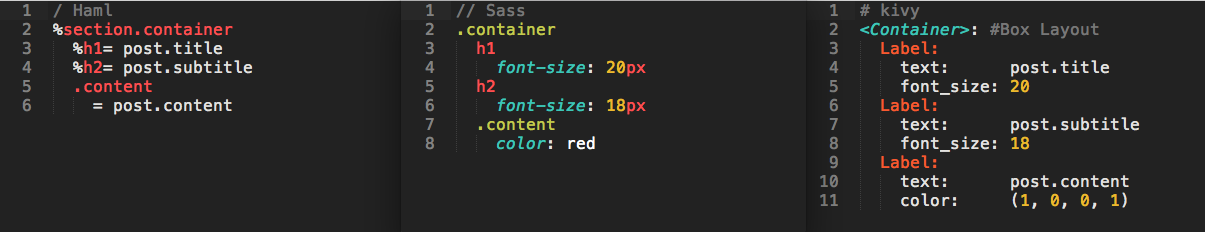
\includegraphics[width=15cm]{images/hamlsasskv.png}
    		\caption{Vergleich zwischen Haml Sass und kv}
    		\label{img:HamlSassKv}
		\end{figure}
        
        Man kann in \emph{kv} zwar auf \emph{Python}-Ausdrücke und Variablen zugreifen, aber alle Arten von Kontrollfluss  – wie z. B. Schleifen – stehen nicht zur Verfügung. So kann eine Liste von Buttons mit der Länge aller gefundenen Wortvorschläge nicht allein in \emph{kv} beschrieben werden. Als Lösung hierfür wurde in dieser Arbeit die Oberfläche in einzelne Module zerlegt. Jedes Modul hat eine eigene Klasse und dazu eine eigene \emph{kv} Datei. Die \emph{Python}-Klasse übernimmt so die Aufgabe eines Controllers, während die \emph{kv} Datei den View beschreibt. Allerdings werden immer noch viele Teile des Views im Controller instanziiert.
        
	\newpage
    \subsection{Wortschatz Verwaltung}
	\subsection{Kathegorisierung}
	\subsection{Wortvorhersage}
    \newpage
    \section{Tests}
	korrekte wort prediction (end to end) wird nicht automatisiert getestet. 
    -> test garantieren unveränderte aber nicht "richtige" vorhersage.
    -> manueller test relativ unkompliziert
    -> genau so clusterer
    
    -> should unit test tokenizer and word predictor
    
    Funktion user interface kann end to end getestet werden
    -> kivy hat kein eigenes ene to end test framework
    -> tests based on this gist
    \newpage
       
	\section{Ergebniss und Resuemee}
    
    Mit den doch sehr kleinen \emph{Corpora} und den daraus generierten \emph{Sprachmodellen} \emph{Märchen} und \emph{Prosa} ist zwar eine Sinnvolle Textvorhersage zu erkennen, diese ist leider aber bei weitem nicht gut genug um tatsächlich ohne weitere Eingaben Sätze zu generieren. Es wäre denkbar darum auf Wunsch eine Tastatur einzublenden und die Vorhersage durch eingegebene Buchstaben zu optimieren. Damit würde die Applikation allerdings auch ein wenig komplexer in der Bedienung werden. 
    
    Mit dem \emph{Sprachmodell} \emph{Simple} können dagegen durchaus sinnvolle Sätze generiert werden. Allerdings sind das Vokabular und auch die möglichen Sätze in diesem \emph{Sprachmodell} natürlich auch viel eingeschränkter. Dies ist zunächst ein durchaus gewolltes Resultat, da man diese Einschränkungen durch wechseln der Kathegorien überwinden kann. Um auf diese Weise eine Nutzbare Software zu generieren müssten allerdings mehrere thematisch unterschiedliche \emph{Corpora} manuell erstellt werden. Möglicherweise ließen sich auch z. B. in Schulbüchern oder Bücher zum erlernen der deutschen Sprache als Corpora nutzbare Texte finden.
    
	Der in \autoref{sec:brownClustering} vorgestellte \emph{Brown Cluster} Algorithmus kann als die in \emph{\autoref{sec:requirements_categories}} geforderte Kategorieerkennung gesehen werden. Allerdings werden hierbei lediglich \emph{bigramms} verwendet. Dies bedeutet, dass die Kategorieauswahl lediglich auf dem vorherigen Wort basiert. Dies ist auch an der Vorhersage deutlich zu merken. So wird in der Kategorie \emph{Prosa} auf den Satzanfang \texttt{ich habe} wieder \texttt{ich} als Wahrscheinlichster Nachfolger vorgeschlagen. Es wäre hier interessant ein einfaches \emph{3-gramm} Modell oder mehrere Algorithmen in Kombination zu testen. \cite{speechcommunication:exchange} beschreiben für ihren \emph{exchange Algorithmus} auch eine Implementierung in welcher \emph{3-gramms} verwendet werden. Auch hier wäre es interessant Ergebnisse zu vergleichen.
            
    Wie in \autoref{sec:input-devices} vorgestellt, wird in der Unterstützen Kommunikation auch viel mit Symbolen gearbeitet. Es kann also davon ausgegangen werden, dass eine große Nutzergruppe Software die textbasiert ist gar nicht bedienen kann. Darum wäre es wünschenswert auch in dem Prototypen mit Symbolen zu arbeiten. Dazu müssten zunächst alle in allen \emph{Corpora} enhaltenen Worte entsprechenden Symbolen zugeordnet werden und diese dann in der Benutzeroberfläche über diesen Worten angezeigt werden. Eine manuelle Einschränkung des Wortschatzes wäre hier unumgänglich. Weitere Anpassungen am Prototypen wären dazu nicht nötig. Das verwenden von Symbolen wäre auch desshalb interessant, da es wie in \autoref{sec:software-examples} gezeigt, bereits gute Lösungen zur Wortvorhersage gibt. In Symbolbasierter Software sind mir allerdings keine solche Lösungen bekannt.
        
        Zusammenfassend lässt sich sagen, das der Prototyp in seiner jetzigen Form leider nicht als \emph{Talker} zu benutzen ist. In der Wortvorhersage gibt es noch viele mögliche und nötige optimierungen. Die verschiedenen \emph{Sprachmodelle} als eigne Kategorien, sind in Ihrer Vorhersage deutlich zu unterscheiden. Gerade das Modell \emph{Simple} zeigt, dass die ursprüngliche Idee den Wortschatz einzuschränken um die Prädiktion zu verbessern im Prinzip funtioniert.  
        
        
           \newpage
    
    %bibliography
    \printbibliography
    \newpage
    
    \appendix
    \renewcommand\thefigure{A.\arabic{figure}}
    \renewcommand*{\thepage}{A\arabic{page}}
    \setcounter{page}{1}
    \setcounter{figure}{0}
    \section*{Annhang}
	\subsection*{Daten}
    	\begin{figure}[H]
			\centering       
			\begin{tabular}{ r || c | c | c}
            	blub & NLP & Natural Language & Natural Language Processing \\ \hline \hline
                Python & 1168 & 500 & 348\\ \hline
                Java & 740 & 269 & 172\\ \hline
                JavaScript & 135 & 146 & 37 \\ \hline
                Ruby & 103 & 100 & 28 \\ \hline
                C++ & 76  & 45 & 23 \\ \hline
			\end{tabular}
        	\caption{caption}
			\label{tab:zzz}
		\end{figure}
    \subsubsection*{Code}

\end{document}